\documentclass[mat1]{fmfdelo}
% \documentclass[fin1]{fmfdelo}
% \documentclass[isrm1]{fmfdelo}
% \documentclass[mat2]{fmfdelo}
% \documentclass[fin2]{fmfdelo}
% \documentclass[isrm2]{fmfdelo}

\usepackage{graphicx}


% naslednje ukaze ustrezno napolnite
\avtor{Maruša Oražem}

\naslov{Konstrukcija gibanja kamere s pomočjo Pitagorejskih krivulj}
\title{Construction of camera motion with help of Pitagorean curves}

% navedite ime mentorja s polnim nazivom: doc.~dr.~Ime Priimek,
% izr.~prof.~dr.~Ime Priimek, prof.~dr.~Ime Priimek
% uporabite le tisti ukaz/ukaze, ki je/so za vas ustrezni
\mentor{izr. prof. dr. Marjetka Knez}
% \mentorica{}
% \somentor{}
% \somentorica{}
% \mentorja{}{}
% \mentorici{}{}

\letnica{2020} % leto diplome

%  V povzetku na kratko opišite vsebinske rezultate dela. Sem ne sodi razlaga organizacije dela --
%  v katerem poglavju/razdelku je kaj, pač pa le opis vsebine.
\povzetek{}

%  Prevod slovenskega povzetka v angleščino.
\abstract{}

% navedite vsaj eno klasifikacijsko oznako --
% dostopne so na www.ams.org/mathscinet/msc/msc2010.html
\klasifikacija{}
\kljucnebesede{} % navedite nekaj ključnih pojmov, ki nastopajo v delu
\keywords{} % angleški prevod ključnih besed

\zapisiMetaPodatke  % poskrbi za metapodatke in veljaven PDF/A-1b standard

% aktivirajte pakete, ki jih potrebujete
% \usepackage{tikz}

% za številske množice uporabite naslednje simbole
\newcommand{\R}{\mathbb R}
\newcommand{\N}{\mathbb N}
\newcommand{\Z}{\mathbb Z}
\newcommand{\C}{\mathbb C}
\newcommand{\Q}{\mathbb Q}
\newcommand{\HH}{\mathbb H}
\newcommand{\rr}{\boldsymbol r}
\newcommand{\ii}{\boldsymbol i}
\newcommand{\jj}{\boldsymbol j}
\newcommand{\kk}{\boldsymbol k}
\newcommand{\pp}{\boldsymbol p}
\newcommand{\ba}{\boldsymbol A}
\newcommand{\e}{\boldsymbol e}
\newcommand{\oo}{\boldsymbol o}
\newcommand{\uu}{\boldsymbol u}
\newcommand{\vv}{\boldsymbol v}
\newcommand{\A}{\mathcal A}
\newcommand{\B}{\mathcal B}
\newcommand{\QQ}{\mathcal Q}
\newcommand{\ff}{\boldsymbol f}
\newcommand{\g}{\boldsymbol g}
\newcommand{\TT}{\boldsymbol T}
\newcommand{\NN}{\boldsymbol N}
\newcommand{\BB}{\boldsymbol B}

% matematične operatorje deklarirajte kot take, da jih bo Latex pravilno stavil
% \DeclareMathOperator{\conv}{conv}

% vstavite svoje definicije ...
%  \newcommand{}{}

\begin{document}

\section{Uvod}

%%%%%%%%%%%%%%%%%%%%%%%%%%%%%%%%%%%%%%%%%%%%%%%%%%%%%%%%%%%%%%%%%%%%%%%%%%%%%%%%%%%%%%%%%%%%%%%%%%%%%%%%
\section{Osnovni pojmi in definicije}
Za začetek, se spoznajmo z osnovnimi pojmi in definicijami, ki jih bomo potrebovali v nadaljevanju.
\begin{definicija}
Množica kvaternioniv $\HH$ je 4-razsežen vektorski prostor z bazo $\bf{1},\bf{i},\bf{j},\bf{k}$.
\end{definicija}
Za $h\in \HH$ pišemo: $h = a + b\mathbf{i} + c\mathbf{j} + d\mathbf{k}$ oziroma $h=(a,b,c,d)$, kjer so $a,b,c,d\in \R$.
Poglejmo si osnovne operacije v množici $\HH$:\\
Seštevanje:
\begin{equation*}
\begin{array}{c c c}
h_1 = (a_1,b_1,c_1,d_1) \in \HH &  \rightarrow & h_1 + h_2 = (a_1+a_2,b_1+b_2,c_1+c_2,d_1+d_2) = \\
h_2 = (a_2,b_2,c_2,d_2) \in \HH &  & (a_1+a_2) + (b_1+b_2)\mathbf{i} + (c_1+c_2)\mathbf{j} + (d_1+d_2)\mathbf{k}
\end{array}
\end{equation*}
Skalarno množenje:
\begin{equation*}
\begin{array}{c c c}
\lambda \in \R, h \in \R & \rightarrow & \lambda h = (\lambda a, \lambda b, \lambda c, \lambda d) =  \lambda a + \lambda b \mathbf{i} + \lambda c \mathbf{j} + \lambda d \mathbf{k}
\end{array}
\end{equation*}
Konjugacija:
\begin{equation*}
\begin{array}{c c c}
h \in \HH & \rightarrow &\overline{h} = (a,-b,-c,-d)= a-b\mathbf{i} - c\mathbf{j} - d\mathbf{k}
\end{array}
\end{equation*}
Kvaternionsko množenje:\\
$\text{Velja zveza:}~\mathbf{i}^2 = \mathbf{j}^2 = \mathbf{k}^2 = \mathbf{ijk} = -1$. Iz te zveze sledijo formule za posamezno množenje dveh baznih elementov. Kvaternion lahko zapišemo kot skalarni in vektorski del. Tako dobimo formulo za množenje dveh kvaternionov:

\begin{equation*}
\begin{split}
& A,B \in \HH \\
&A = (a, \boldsymbol{a}), ~~ a,b \in \R \\
&B = (b, \boldsymbol{b}), ~~ \boldsymbol{a}, \boldsymbol{b} \in \R^3\\
A\cdot B = & \left( ab- \langle \boldsymbol{a},\boldsymbol{b} \rangle, a\boldsymbol{b}-b\boldsymbol{a}-\boldsymbol{a}\times \boldsymbol{b}  \right)
\end{split}
\end{equation*}
Zaradi lažjega razumevanja, bomo kvaternionsko množenje označevali z $\cdot$, skalarno množenje pa $\langle\cdot,\cdot\rangle$.
\begin{primer}
	Primer uporabe formule za kvaternionsko množenje. Izpeljali bomo formulo za skalarno množenje dveh kvaternionov, ki imata skalarni del enak 0.
	Vemo:
	\begin{equation*}
	A\cdot B =  \left( ab- \langle \boldsymbol{a},\boldsymbol{b} \rangle, a\boldsymbol{b}-b\boldsymbol{a}-\boldsymbol{a}\times \boldsymbol{b}  \right)
	\end{equation*}
	Naj bosta sedaj $A = (0,\boldsymbol{a})$ in $(0,\boldsymbol{b})$. Dobimo:
	\begin{equation*}
	(0,\boldsymbol{a}) \cdot (0,\boldsymbol{b}) = \left( -\langle \boldsymbol{a}, \boldsymbol{b} \rangle , -\boldsymbol{a} \times \boldsymbol{b} \right)
	\end{equation*}
	Iz česar sledi:
	\begin{equation*}
	\langle \boldsymbol{a},\boldsymbol{b} \rangle = -scal\left( (0,\boldsymbol{a}) \cdot (0,\boldsymbol{b}) \right)
	\end{equation*}
\end{primer}
Norma kvaterniona:
\begin{equation*}
\begin{array}{c c}
h \in \HH & \rightarrow ||h|| = \sqrt{\langle h, \overline{h}\rangle}
\end{array}
\end{equation*}
\begin{definicija}
Krivulja $\rr$ je \textit{racionalna}, če velja $\rr(t) = \frac{p(t)}{q(t)}$, kjer sta $p$ in $q$ polinoma.
\end{definicija}
\begin{definicija}
\textit{Parametrično podana krivulja} v $\R^n$ je množica točk, podana s parametrizacijo:
\begin{equation*}
\rr: [ a,b ] \rightarrow \R^n
\end{equation*}
\begin{equation*}
t ~ \longmapsto ~\rr(t)
\end{equation*}
\end{definicija}
\begin{primer}
n = 3:
\begin{equation*}
\rr:[a,b] \rightarrow \R^3
\end{equation*}
\begin{equation*}
t \longmapsto \rr(t) = (x(t),y(t),z(t))
\end{equation*}
\end{primer}
\begin{definicija}
Parametrično podana krivulja $\rr$ je \textit{Pitagorejska krivulja\\ (P-krivulja)}, če je $\boldsymbol{o}(t) = \frac{\rr(t)}{||\rr(t)||}$ .
\end{definicija}
\begin{opomba}
Dovolj je zahtevati (na primer za $n = 3$), da je\\ $||\rr(t)|| = \sqrt{x(t)^2 + y(t)^2 + z(t)^2}$ polinom, oziroma $x(t)^2 + y(t)^2 + z(t)^2 = \sigma^2$ za nek $\sigma$.
\end{opomba}


%%%%%%%%%%%%%%%%%%%%%%%%%%%%%%%%%%%%%%%%%%%%%%%%%%%%%%%%%%%%%%%%%%%%%%%%%%%%%%%%%%%%%%%%%%%%%%%%%%%%%%%%%%%
\section{Konstrukcija P-krivulje}
V tem razdelku bom opisala postopek, s katerim bomo dobili našo krivuljo.\\
Za začetek vzemimo poljubni kvaternionski polinom $\mathcal{A}(t)$, ki naj bo stopnje $n$. Torej:
\begin{equation*}
\mathcal{A}: I \subset \R \rightarrow \HH
\end{equation*}
\begin{equation*}
\begin{array}{c c c}
\mathcal{A}(t) = u(t) + v(t) \mathbf{i} + p(t) \mathbf{j} + q(t) \mathbf{k}, & t \in I,& u,v,p,q \in \R[t].
\end{array}
\end{equation*}
Iz kvaternionskega polinoma $\mathcal{A}(t)$, bomo konstruirali parametrično krivuljo $\mathbf{p}(t)$. In sicer:
\begin{equation}
\boldsymbol{p}(t) := \mathcal{A}(t) \boldsymbol{i} \overline{\mathcal{A}}(t)
\end{equation}
Pokažimo, da je krivulja dobljena bo zgornjem predpisu, res parametrična krivulja. Izkaže se, da je tudi P-krivulja in sicer stopnje 2n. Zaradi boljše preglednosti, bomo izpustili argument, vendar se zavedamo, da so prepisi odvisni od parametra t.
\begin{equation*}
\begin{array}{c}
\mathcal{A} = u + v\boldsymbol{i} + p \boldsymbol{j} + q \boldsymbol{k}  \\
\overline{\mathcal{A}} = u - v\boldsymbol{i} - p \boldsymbol{j} - q \boldsymbol{k}  \\
\mathcal{A} \boldsymbol{i} = u \boldsymbol{i} + v \boldsymbol{i}^2 + p \boldsymbol{ji} + q\boldsymbol{ki} =  u \boldsymbol{i} - v - p \boldsymbol{k} + q\boldsymbol{j}	
\end{array} 
\end{equation*}
\begin{equation*}
\begin{split}
\mathcal{A}\boldsymbol{i}\overline{\mathcal{A}} & =(u\boldsymbol{i}-v-p\boldsymbol{k}+q\boldsymbol{j})(u-v\boldsymbol{i}-p\boldsymbol{j}-q\boldsymbol{k}) \\
&= u^2 \ii -uv\ii^2-pu\ii\jj - uq\ii\kk - vu + v^2\ii + vp\jj\\
&~~ +vq\kk - pu\kk + pv\kk\ii + p^2 \kk\jj + pq\kk^2 + qu\jj - qv\jj\ii - qp\jj^2 -q^2\jj\kk \\
& = u^2\ii + uv - pu\kk + uq\jj -vu+v^2\ii +vp\jj + vq\kk \\
& ~~-pu\kk+pv\jj-p^2\ii-pq+qu\jj+qv\kk+qp-q^2\ii \\
& = (u^2+v^2-p^2-q^2)\ii + 2(uq-vp)\jj +2(vq-pu)\kk
\end{split}
\end{equation*}
Opazimo, da imao samo 3 bazne elemente, saj je skalarni del enak 0. Zato lahko $\pp = \A\ii\A$ identificiramo z točko v $\R^3$. Torej dobimo:
\begin{equation*}
\pp = (u^2+v^2-p^2-q^2, 2(uq+vp),2(vq-pu)).
\end{equation*}
Na začetku smo vzeli kvaternionski polinom $\A=u+v\ii+p\jj+q\kk$, kjer so $u,v,p,q$ polinomi stopnje n. Ker v $\pp$ nastopajo le zmnožki dveh teh polinom, vsote in razlike, je dobljeni $\pp$ stopnje 2n.\\
Pokažimo sedaj, da je krivulja $\pp$ dobljena po zgornjem predpisu, P-krivulja. Da bo krivulja P-krivulja, mora veljati, da je $\boldsymbol{o} = \frac{\pp}{||\pp||}$ racionalna krivulja. Vemo že, da je $\pp$ polinom. Preverimo, da je tudi $||\pp||$ polinom.
\begin{equation*}
\begin{split}
||\pp||^2 &= \langle \pp,\overline{\pp}\rangle = (\A\ii\overline{\A})\overline{(\A\ii\overline{\A})} \\
&= \A\ii\overline{\A}\A\overline{\ii} \overline{\A} \\
\langle \overline{\A}, \A \rangle = ||\A||^2 ~~ \longrightarrow ~~& = ||\A||^2 \A \ii \overline{\ii} \overline{\A} \\
\ii(-\ii) = -\ii^2 = 1 ~~ \longrightarrow ~~ & = ||\A||^2 \A \overline{\A} \\
&=||\A||^4 \\
\Longrightarrow ~~~~ & ||\pp|| = ||\A||^2
\end{split}
\end{equation*}
Pokazali smo, da je $||\pp|| = ||\A||^2$, vemo pa, da je $\A$ sestavljen iz polinomov. Torej je $||\pp||$ res polinom.\\

Sklep: Iz kvaternionskega polinoma $\A(t)$, stopnje n, smo po predpisu\\ $\pp(t) = \A(t)\ii\overline{\A(t)}$ konstruirali P-krivuljo stopnje 2n. 

\subsection{Zapis krivulje v Bernsteinovi bazi}
Naš cilj je opisati gibanje kamere okoli nekega fiksnega objekta. Želimo si nadzorovati to gibanje in vsaj pribljižno napovedati, kje se bo krivulja gibala. Videli bomo, da tega ne moremo doseči, če krivuljo zapišemo v standardni bazi. To bomo dosegli s pomočjo Bernsteinove baze. \\
Poglejmo si najprej zapis krivulje v standardni bazi. Poljuben polinom $\pp$ stopnje n, se v standardni bazi zapiše kot:
\begin{equation*}
\begin{array}{c c}
\pp(t) = \sum_{i=0}^n p_i t^i & \text{kjer so $p_i$ točke v $\R^3$.}
\end{array}
\end{equation*}
Poglejmo si nekaj preprostih primerov, primerjamo izbrane točke $p_i$ in obliko dobljene krivulje $\pp(t)$.
\begin{equation*}
\begin{array}{c c}
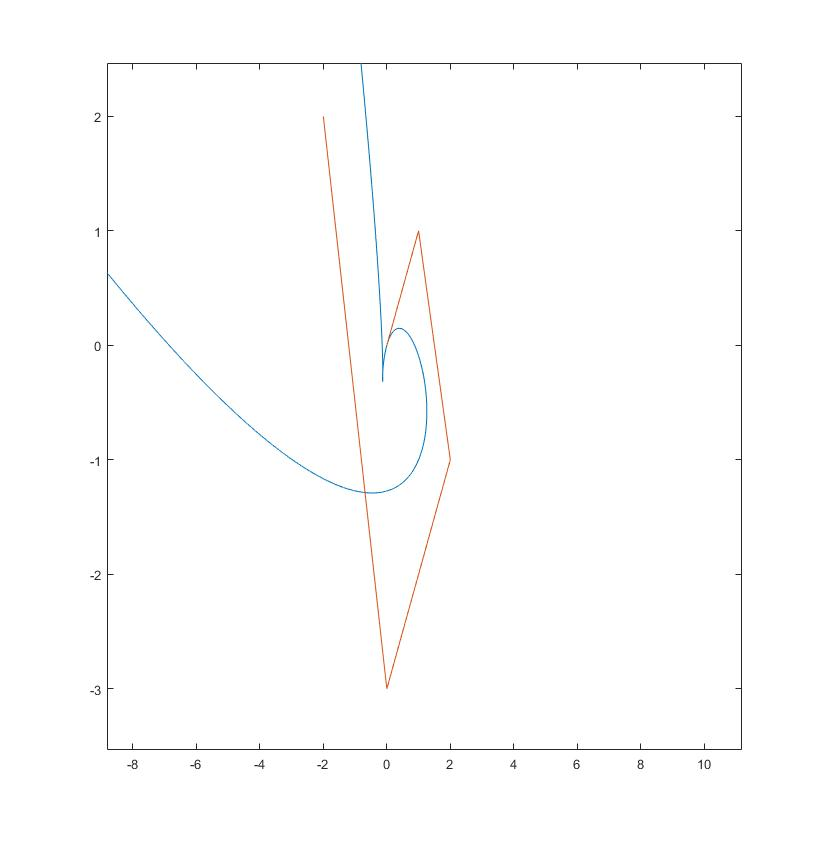
\includegraphics[scale=0.20]{C:/Users/Acer/Desktop/diploma/Diploma/slike/standKrivulja3.jpg} &
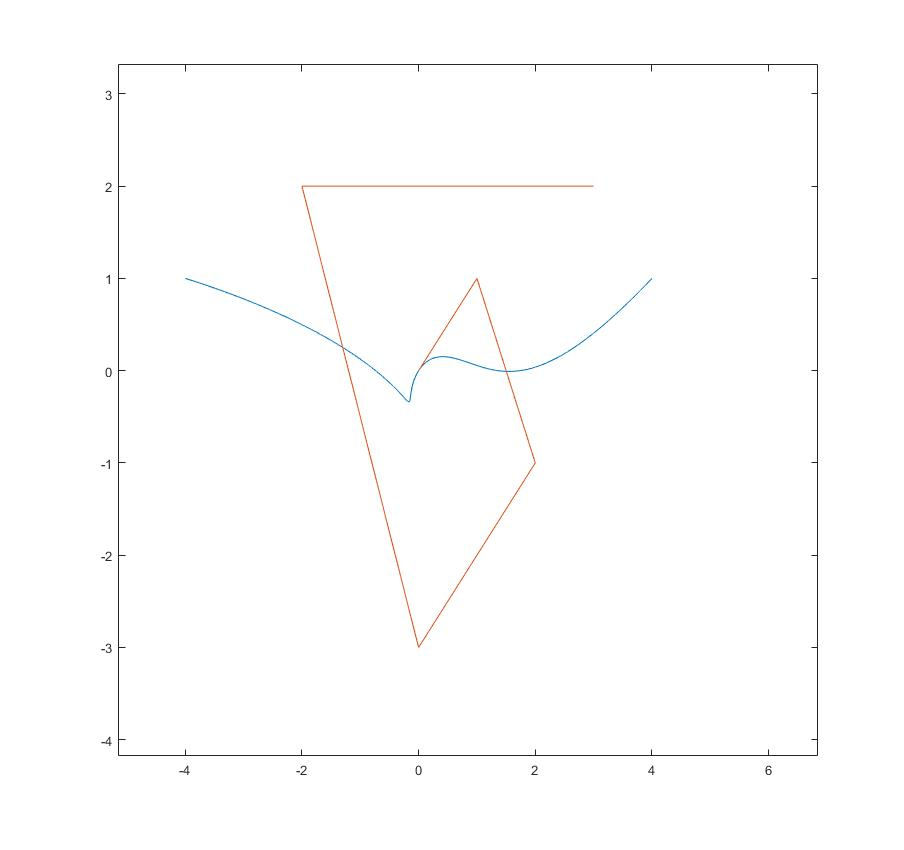
\includegraphics[scale=0.20]{C:/Users/Acer/Desktop/diploma/Diploma/slike/standKrivulja4.jpg}
\end{array}
\end{equation*}
Na zgornjih slikah, so z oranžno barvo narisane in povezane izbrane točke $p_i$, z modro pa
dobljena krivulja $\pp(t)$, zapisana v standardni bazi.
Vidimo, da med izbranimi točkami in obliko krivulje, ni vidne povezave. \\

Poglejmo si, kaj je to Bernsteinova baza in kakšno povezavo imajo točke z obliko krivulje.
\begin{definicija}
Bernsteinovi bazni polinomi, ki tvorijo bazo polinomov stopnje n, so:
\begin{equation*}
\begin{array}{c c}
B_i^n(t) = \binom{n}{i} tî (1-t)^{n-i}, & i=0,1,\dots,n
\end{array}
\end{equation*}
\end{definicija}
\begin{equation*}
\begin{array}{c c}
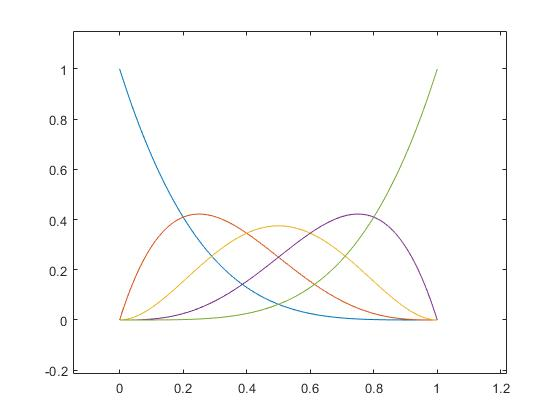
\includegraphics[scale=0.35]{C:/Users/Acer/Desktop/diploma/Diploma/slike/bernPolinom4.jpg} &
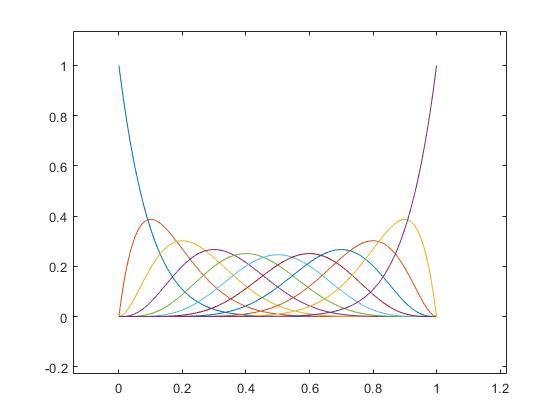
\includegraphics[scale=0.35]{C:/Users/Acer/Desktop/diploma/Diploma/slike/bernPolinom10.jpg}
\end{array}
\end{equation*}
Zgornji sliki sta grafični prikaz Bernsteinovih baznih polinomov za $n = 4$ in $n= 10$.\\


Zapišimo sedaj kvaternionski polinom $\A(t)$ v Bernsteinovi bazi. Dobimo:
\begin{equation*}
\A(t) = \sum_{i=0}^n \boldsymbol{A}_i B_i^n(t),
\end{equation*}
kjer so $\boldsymbol{A}_i \in \HH$ in $B_i^n$ Bernsteinovi bazni polinomi. Točkam $A_i$ rečemo kontrolne točke, te pa tvorijo tako imenovani kontrolni poligon, ki določa obliko krivulje.

\begin{equation*}
\begin{array}{c c}
\includegraphics[scale=0.35]{C:/Users/Acer/Desktop/diploma/Diploma/slike/bernKrivulja1.jpg} &
\includegraphics[scale=0.15]{C:/Users/Acer/Desktop/diploma/Diploma/slike/bernKrivulja3.jpg}
\end{array}
\end{equation*}
Zgornji sliki nam prikazujeta krivuljo, dobljeno iz kontrolnih točk in zapisano v Bernsteinovi bazi. Vidimo, da če si narišemo kontrolni poligon (oranžna barva), se krivulja (modra barva) začne v prvi kontrolni točki in konča v zadnji. Pot krivulje med tema dvema točkama, pa poteka po notranjosti mnogokotnika, ki ga določa kontrolni poligon.
\iffalse
Primer prileganja krivulje kontrolnemu poligoni na točkah (0,0), (1,1), (2,-1), (0,-3), (-2,2) in če dodamo še (3,2).
\fi
\begin{primer}
$n = 2$
\begin{equation*}
B_i^2(t) = \binom{2}{i} t^i(1-t)^{2-i}, ~~ i=0,1,2
\end{equation*}
\begin{equation*}
\begin{split}
B_0^2(t) &= \binom{2}{0} t^0(1-t)^{2-0} = (1-t)^2\\
B_1^2(t) &= \binom{2}{1} t^1(1-t)^{2-1} = 2t(1-t)\\
B_2^2(t) &= \binom{2}{2} t^2(1-t)^{2-2} = t^2\\
\Longrightarrow \A(t) &= \boldsymbol{A}_0(1-t)^2 + \boldsymbol{A}_1 2t(1-t) + \boldsymbol{A}_2t^2
\end{split}
\end{equation*}
\begin{equation*}
\begin{array}{c c}
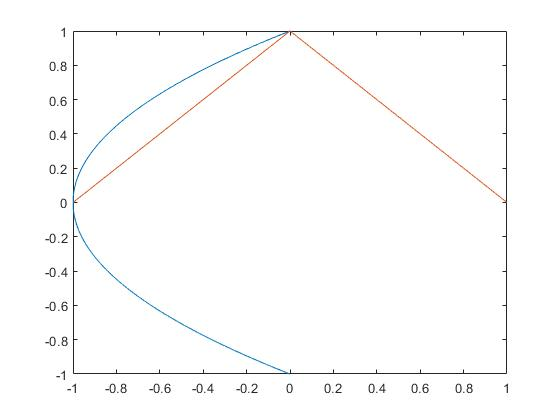
\includegraphics[scale=0.35]{C:/Users/Acer/Desktop/diploma/Diploma/slike/stand3.jpg} &
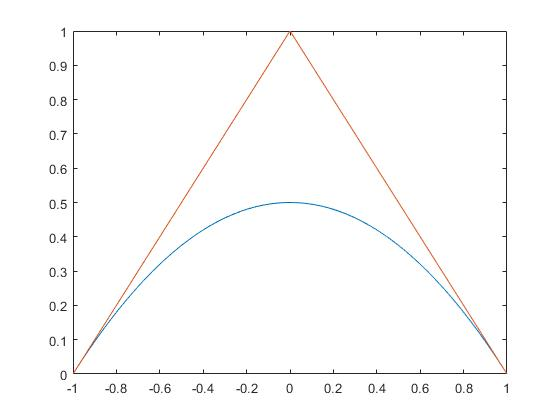
\includegraphics[scale=0.35]{C:/Users/Acer/Desktop/diploma/Diploma/slike/bern3.jpg}
\end{array}
\end{equation*}
Na zgornjih dveh slikah sta prikazani krivulji, ki jih dobimo, če vzamemo enake kontrolne točke in določimo krivuljo v standarni bazi (leva slika) in v Bernsteinovi bazi (desna slika). Kot smo že ugotovili zgoraj, je dobljena oblika lepša, če je krivulja zapisana v Bernsteinovi bazi. Nadzorujemo lahko začetno in končno točko, ter obliko krivulje.
\iffalse
primer polinoma zapisanega v standardni bazi in bernsteinovi bazi, z istimi kontrolnimi točkami (-1,0), (0,1), (1,0).
\fi
\end{primer}



\subsection{Določitev kontrolnih točk}
V tem razdelku, si bomo pogledali, kako določiti kontrolne točke za krivuljo, zapisano v Bernsteinovi bazi. Vprašanje je, kakšni naj bodo začetni koeficienti polinoma $\A(t)$, če določimo koeficiente krivulji $\pp(t)$. Torej, izbrane imamo točke, ki nam določajo obliko poti krivulje. Kakšni naj bodo potem koeficienti začetnega polinoma $\AA(t)$?
\begin{primer}
$n=1$
\begin{equation*}
\begin{split}
\text{Bernsteinova baza}:&~~ B_i^1(t) = \binom{1}{i} t^i(1-t)^{1-i}, ~~ i= 0,1 \\
B_0^1(t) &= \binom{1}{0} t^0(1-t)^{1-0} = 1-t \\
B_1^1(t) &= \binom{1}{1} t^1(1-t)^{1-1} = t \\
\Longrightarrow \A(t) &= \boldsymbol{A}_0(1-t) + \boldsymbol{A}_1t
\end{split}
\end{equation*}

Rekli smo, da je $\pp(t) = \A \ii \overline{\A}$. Vemo, da se splošni polinom stopnje n, v Bernsteinovi bazi, zapiše kot:
\begin{equation*}
\pp(t) = \sum_{k=0}^n p_k \binom{n}{k}(1-t)^{n-k}t^k.
\end{equation*}
Pokazali smo, da če je $\A$ stopnje $n$, bo $\pp = \A\ii\overline{\A}$ stopnje $2n$.Torej
\begin{equation*}
\begin{split}
B_0^2(t)& = (1-t)^2\\
B_1^2(t) &= 2t(1-t)\\
B_2^2(t) &= t^2 \\
\Longrightarrow \pp(t) = \sum_{i=0}^2 \pp_i B_i^2 &= \pp_0 (1-t)^2 + \pp_12t(1-t) + \pp_2t^2
\end{split}
\end{equation*}
Računamo:
\begin{equation*}
\begin{split}
\pp(t) &= \A(t)\ii\overline{\A(t)} \\
&= (\boldsymbol{A}_0(1-t) + \boldsymbol{A}_1t) \ii ( \overline{\boldsymbol{A}_0}(1-t) + \overline{\boldsymbol{A}_1}t) \\
& = (\boldsymbol{A}_0(1-t) + \boldsymbol{A}_1t) (\ii\overline{\boldsymbol{A}_0}(1-t) + \ii\overline{\boldsymbol{A}_1}t) \\
&=\ba_0 \ii \overline{\ba_0} (1-t)^2 + \ba_0\ii\overline{\ba_1}(1-t)t + \ba_1\ii\overline{\ba_0}t(1-t) + \ba_1\ii\overline{\ba_1}t^2 \\
&= \ba_0 \ii \overline{\ba_0} (1-t)^2 + \left(\frac{1}{2}\ba_0\ii\overline{\ba_1} +\frac{1}{2} \ba_1\ii\overline{\ba_0}\right)2t(1-t) + \ba_1\ii\overline{\ba_1}t^2
\end{split}
\end{equation*}
Primerjamo istoležne koeficiente in dobimo naslednje enačbe:
\begin{equation*}
\begin{split}
\pp_0&= \ba_0\ii\overline{\A_0} \\
\pp_1&= \frac{1}{2}\left( \ba_0\ii\ba_1\overline{\A_1} + \A_1\ii\overline{\A_0}\right)\\
\pp_2&= \ba_1\ii\overline{\A_1}\end{split}
\end{equation*}
\end{primer}
Z analognim računom pridemo do točk za polinome višjih stopenj.
\begin{primer}
$n=2$ ($\pp$ bo stopnje 4).
\begin{equation*}
\begin{split}
\A(t) &= \ba_0(1-t)^2 + \ba_12t(1-t) + \ba_2(1-t)^2\\
\pp(t)& = \sum_{k=0}^4\pp_iB_i^4(t) \\
\Longrightarrow ~~\pp_0 & = \ba_0\ii\overline{\A_0} \\
\pp_1 &= \frac{1}{2}\left( \ba_0\ii\overline{\A_1} + \ba_1\ii\overline{\A_0} \right) \\
\pp_2 &= \frac{1}{6} \left( \ba_0\ii\overline{\A_2} + 4\ba_1\ii\overline{\A_1}+\ba_2\ii\overline{\A_0} \right) \\
\pp_3 &= \frac{1}{2} \left( \ba_1\ii\overline{\A_2}+\ba_2\ii\overline{\A_1} \right) \\
\pp_4 &= \ba_2\ii\overline{\A_2}
\end{split}
\end{equation*}
\end{primer}
\iffalse
Z višanjem stopnje začetnega polinoma, dobimo več prostih parametrov, kar lahko izkoristimo pri konstrukciji krivulje. Več o tem kasneje.
\fi
Sedaj, ko imamo poračunane kontrolne točke, lahko iz njih poračunamo začetne koeficiente polinoma $\A$. Na primer, lahko si izberemo začetno in končno točko krivulje $\pp(0)$ in $\pp(1)$.
\begin{primer}
	$n=1$
	\begin{equation*}
	\begin{split}
		\ba_0\ii\overline{\A_0} &= \pp(0) \\
		\ba_1\ii\overline{\A_1} &= \pp(1)
	\end{split}
\end{equation*}
Iz teh dveh enačb, lahko izrazimo $\ba_0$ in $\ba_1$ in dobimo začetni kvaternionski polinom $\A$. Podobno za polinome višjih stopenj, kjer si lahko izberemo začetno in končno točko, ter še dodatno točko.	
\end{primer}
%%%%%%%%%%%%%%%%%%%%%%%%%%%%%%%%%%%%%%%%%%%%%%%%%%%%%%%%%%%%%%%%%%%%%%%%%%%%%%%%%%%%%%%%%%%%%%%%%%%%%%%%%%%%%%%%%%%%%%%%%%%%%%%%%%%
\section{Ogrodja}

\subsection{Usmerjena in prikrojena ogrodja}
Pogledali si bomo, kakšna je razlika med usmerjenimi in prikrojenimi ogrodji.
\begin{definicija}
	Ogrodje $(\e_1,\e_2,\e_3)$ je prikrojeno, če se $\e_1$ v vsaki točki krivulje ujema z enotsko tangento, $\e_2$ in $\e_3$ pa v vsaki točki napenjata normalno ravnino.
\end{definicija}
\begin{primer}
	Nam najbolj znan primer prikrojenega ogrodja, je Frenetovo ogrodje. To ogrodje je tako znano, da ima tudi svoje oznake. Ogrodje, na parametrični krivulji $\rr(t)$, označimo z $(\TT,\NN,\BB)$, kjer so posamezni vektorji definirani kot:
	\begin{equation*}
		\begin{array}{c c c}
		\TT = \frac{\rr'}{|\rr'|},~ & \NN = \frac{\rr' \times \rr''}{|\rr' \times \rr''|} \times \TT,~ &
		\BB = \frac{\rr' \times \rr''}{|\rr' \times \rr''|}
		\end{array}
	\end{equation*}
	\begin{equation*}
	\begin{array}{c c}
	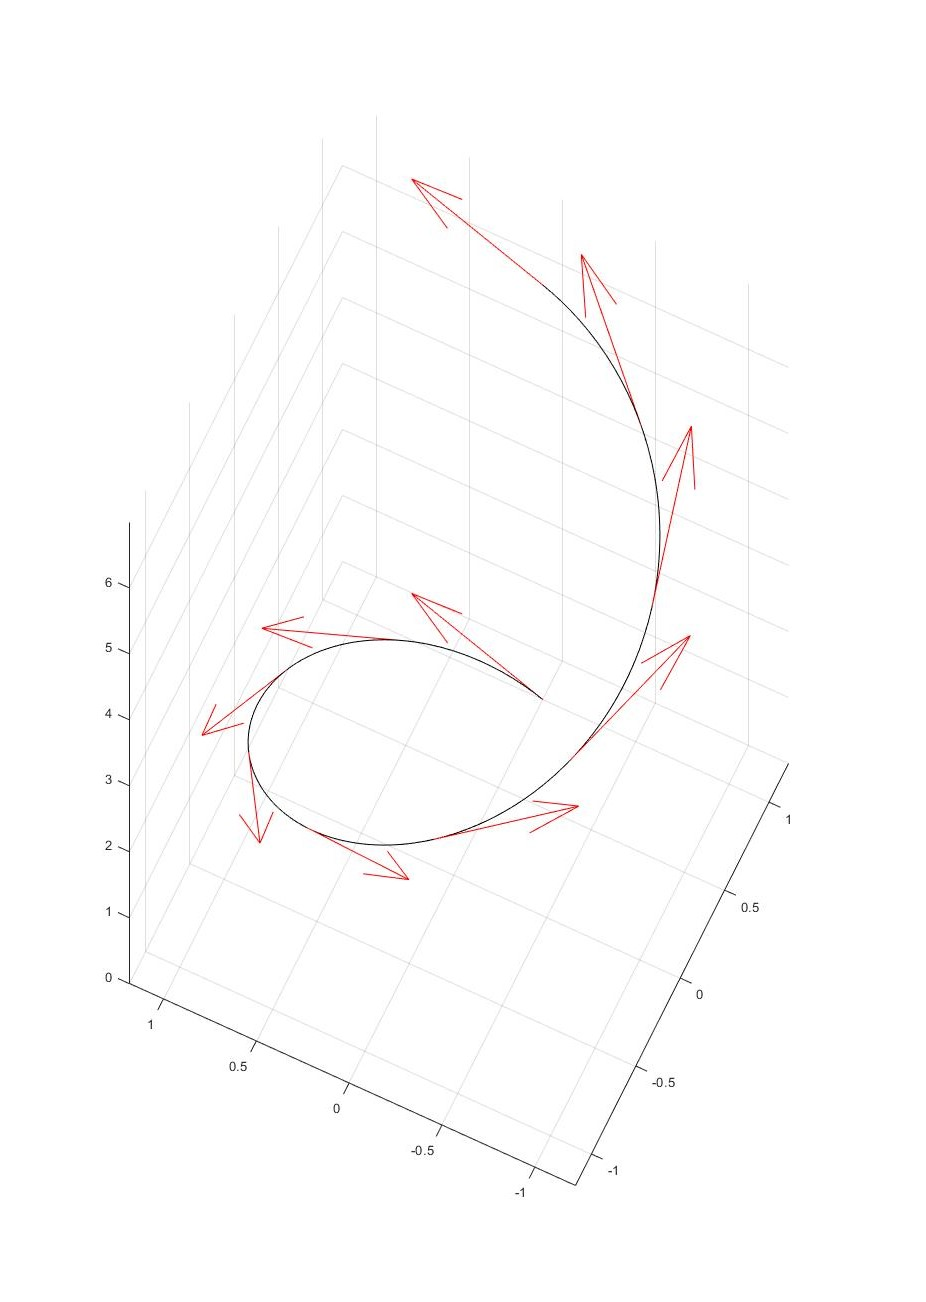
\includegraphics[scale=0.2]{C:/Users/Acer/Desktop/diploma/Diploma/slike/FrenetOgrodjeTangenta'.jpg} &
	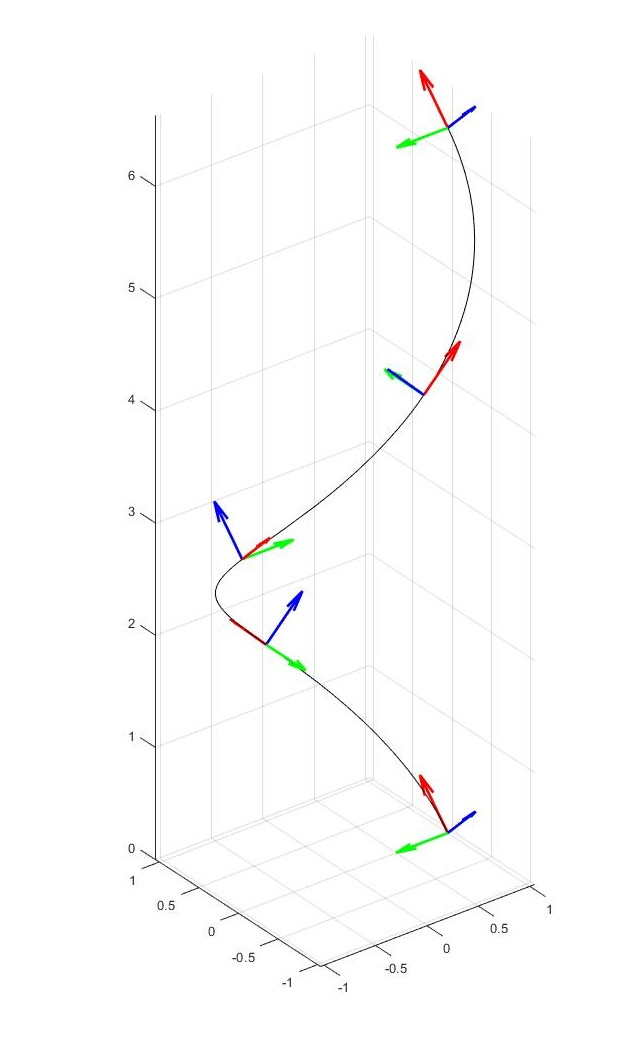
\includegraphics[scale=0.25]{C:/Users/Acer/Desktop/diploma/Diploma/slike/FrenetOgrodjeBold'.jpg}
	\end{array}
	\end{equation*}
	Na zgornji levi sliki je prikazan tangentni vektor, na levi pa krivulja z Frenetovim ogrodjem.
\end{primer}
\begin{definicija}
Ogrodje $(\e_1,\e_2,\e_3)$ je usmerjeno, če $\e_1$ v vsaki točki krivulje kaže proti izhodišču.
\end{definicija}
\begin{equation*}
\begin{array}{c c}
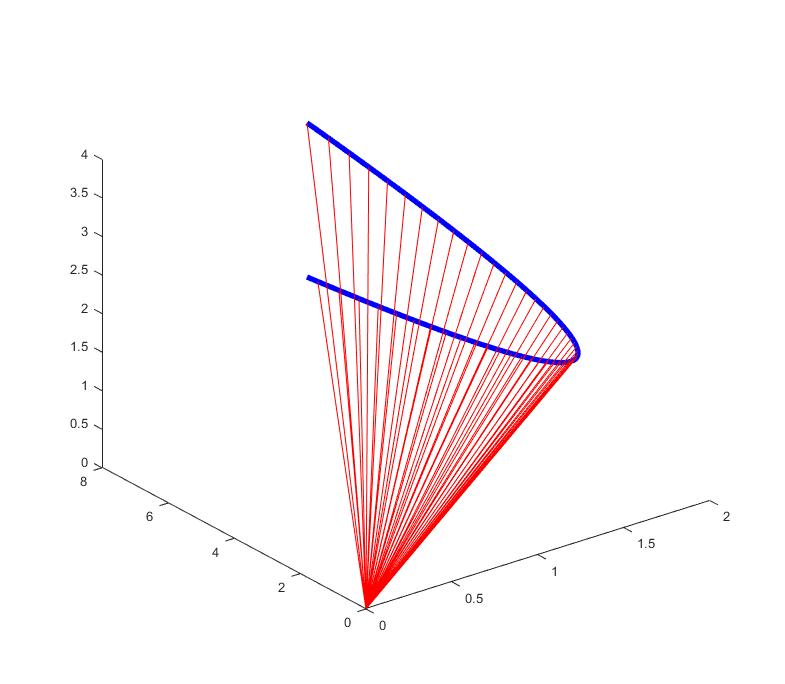
\includegraphics[scale=0.25]{C:/Users/Acer/Desktop/diploma/Diploma/slike/polarindi1.jpg} &
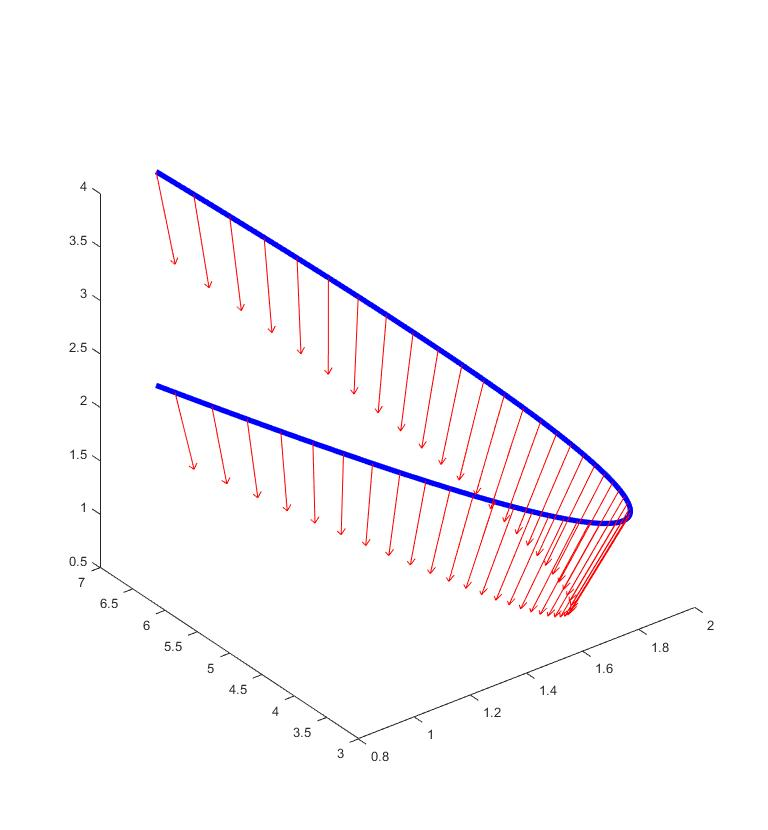
\includegraphics[scale=0.25]{C:/Users/Acer/Desktop/diploma/Diploma/slike/polarindi4.jpg}
\end{array}
\end{equation*}
Na zgornjih slikah vidimo krivuljo in vektor $\e_1$, ki vedno kaže proti izhodišču. 
\begin{opomba}
	Vektor $\e_1$ imenujemo polarni indikator.
\end{opomba}
Sedaj ko smo si pogledali obe vrsti ogrodij, je seveda logično, katero ogrodje si bomo izbrali pri naši konstrukciji. Ker si želimo opisati gibanje kamere, ki bo ves čas potovanje po krivulji snemala nek fiksen objekt v izhodišču, si izberemo usmerjeno ogrodje in položaj kamere orientiramo skladno z danim ogrodjem.

\subsection{Rotacijsko minimizirajoča ogrodja} Pojem se povezuje z dejstvom, da si želimo čim manj nepotrebnih rotacij samega ogrodja. Bolj natančno, vektorja $\e_2$ in $\e_3$, ki razpenjata normalno ravnino, naj nimata nobene nenadne rotacije okoli vektorja $\e_1$. Poglejmo si primer na Frenetovem ogrodju.
\begin{primer}
	Mislimo si, da je vektor $\TT$ fiksiran. V vsaki točki krivulje imamo 2 enotska tangentna vektorja, v vsaki točki izberemo enako orientacijo. Kaj pa druga dva vektorja? Problem je v tem, da lahko druga dva vektorja zarotiramo za poljuben kot, tako dobljeni vektorji, pa še vedno tvorijo ogrodje. Torej vektorja $\e_2$ in $\e_3$ lahko izberemo kot poljubni rotaciji vektorjev $\NN$ in $\BB$, za poljuben kot $\phi$.
	\begin{equation*}
		\begin{bmatrix}
		\e_2 \\
		\e_3
		\end{bmatrix}
		=
		\begin{bmatrix}
		cos \phi & sin \phi \\
		-sin \phi & cos \phi
		\end{bmatrix}
		\begin{bmatrix}
		\NN \\ \BB
		\end{bmatrix}
	\end{equation*}
\begin{equation*}
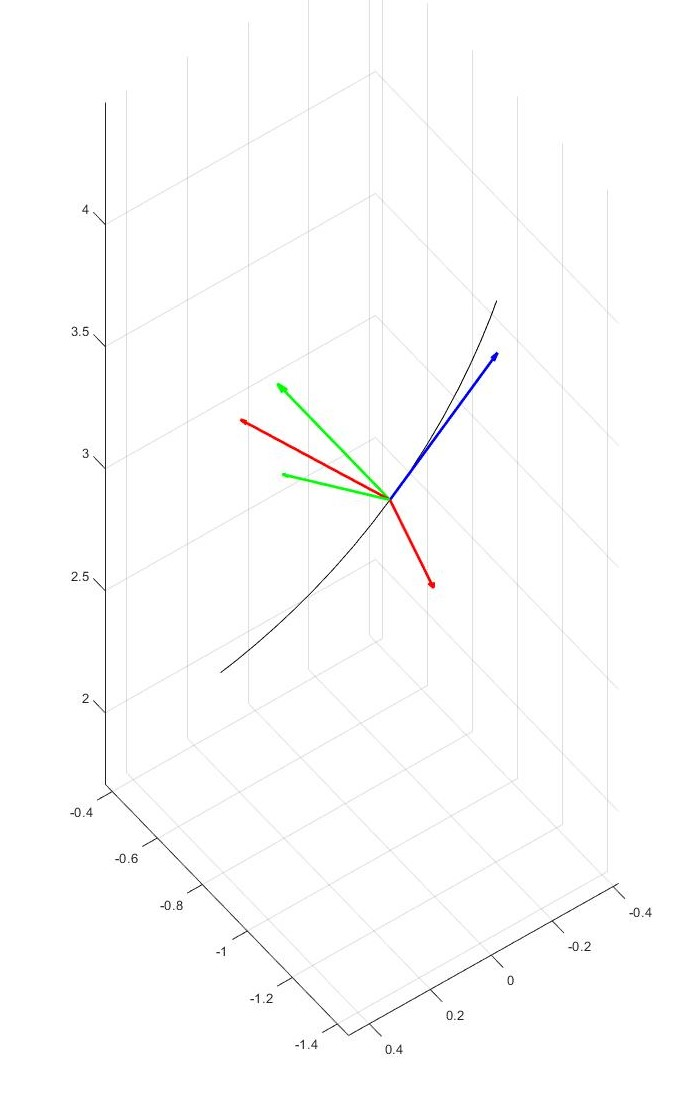
\includegraphics[scale=0.25]{C:/Users/Acer/Desktop/diploma/Diploma/slike/dvaOgrodja'.jpg}
\end{equation*}
Na zgornji sliki vidimo tak primer. Modri tangentni vektor $\TT$, in zelena $\NN$ in $\BB$ tvorijo Frenetovo ogrodje. Vendar prav tako tvorijo Frenetovo ogrodje moder vektor $\TT$ in rdeča $\NN$ in $\BB$.
\end{primer}
Torej, izmed vseh možnih ogrodij, ki jih lahko konstruiramo na krivulji, nas bodo zanimala le taka, ki nam zagotovijo čim manj rotacij v ravnini, ki je pravokotna  na $\e_1$.
 
Vsako ogrodje ima neko kotno hitrost $\omega$, ki nam pove, kako se ogrodje spreminja, oziroma kako se spreminjata vektorja $\e_2$ in $\e_3$.
\begin{definicija}
Naj bo $(\e_1,\e_2,\e_3)$ ogrodje in $\omega$ pripadajoča kotna hitrost. Potem je $\omega$ definirana z naslednjimi diferencialnimi enačbami:
\begin{equation}
\frac{de_i}{dt}(t) = \omega(t) \times e_i(t), ~~ i=1,2,3.
\end{equation}
\end{definicija}

Ker se bomo v nadaljevanju ukvarjali samo z usmerjenimi ogrodji, si poglejmo povezavo med le temi.
\begin{definicija}
Usmerjeno ogrodje $(\e_1,\e_2,\e_3)$ je rotacijsko minimizirajoče, če velja $\langle \omega,\e_1\rangle = 0.$
\end{definicija}

\begin{trditev}
Ogrodje $(\e_1,\e_2,\e_3)$, definirano kot: 
\begin{equation*}
\begin{array}{c c c}
\e_1 = \frac{\A\ii\overline{\A}}{\A\overline{\A}}, &
\e_2 = \frac{\A\jj\overline{\A}}{\A\overline{\A}}, &
\e_3 = \frac{\A\kk\overline{\A}}{\A\overline{\A}}
\end{array}
\end{equation*}
je ortonormirana baza prostora $\R^3$.
\end{trditev}
\begin{dokaz}
Pokazati moramo, da so skalarni produkti $\langle \e_i, \e_j \rangle $ enaki 0, za $i, j = 1,2,3, i \neq j$. Vemo, da so skalarni deli $\e_1,\e_2,\e_3$ enaki 0, zato lahko uporabimo formulo za skalarni produkt dveh "čistih" kvaternionov.
\begin{equation*}
\begin{split}
	\langle \e_1,\e_2 \rangle& = -scal \left( \e_1 \cdot \e_2 \right) \\
	& = -scal \left( \A \ii \overline{\A} \A \jj \overline{\A} \right) \\
	&= - ||\A||^2 scal \left( \A \ii \jj \overline{\A} \right) \\
	& = - ||\A||^2 scal \left( \A \kk \overline{\A} \right) \\
	& = 0
\end{split}
\end{equation*}
Analogno poračunamo $\langle \e_2,\e_3 \rangle$, $\langle \e_1,\e_3 \rangle$.
Izračunajmo še njihove dolžine.
\begin{equation*}
\begin{split}
\A \ii \overline{\A} \A \ii \overline{\A} 	&= ||A||^2 \A \ii^2 \overline{\A} \\
	&= -||A||^4 \\
	\Longrightarrow \langle \e_1,\e_1 \rangle &= -scal \left( \e_1 \cdot \e_1 \right) \\
	&= -scal (-\frac{1}{||\A||^4}||A||^4) \\
	&= 1
\end{split}
\end{equation*}
Analogno poračunamo dolžine vektorjev $\e_2$ in $\e_3$. Torej je to res ortonormirana baza $\R^3$.
\end{dokaz}
\begin{trditev} Recimo, da imamo ogrodje definicirano kot zgoraj.
	Usmerjeno ogrodje je rotacijsko minimizirajoče $\Leftrightarrow$ ko je $scal(\A' i\overline{\A})\equiv0$.
\end{trditev}
\begin{opomba}
	Oznaka $scal(\cdot)$ označuje skalarni del produkta.
\end{opomba}
\begin{dokaz}
Želimo pokazati, da velja:
\begin{equation}
\langle \omega,\e_1\rangle = 0 \Leftrightarrow scal(\A' \\i\overline{\A}) = 0.
\end{equation}
Razvijemo $\omega$ po bazi: $\omega = \omega_1\e_1+\omega_2\e_2+\omega_3\e_3$. \\
Računamo:
\begin{equation*}
\begin{split}
0 = \langle \omega, \e_1 \rangle &= \langle \omega_1\e_1,\e_1\rangle + \langle \omega_2\e_2,\e_1\rangle + \langle \omega_3\e_3,\e_1\rangle \\
&= \omega_1\langle \e_1,\e_1\rangle + \omega_2\langle \e_2,\e_1\rangle + \omega_3\langle \e_3,\e_1\rangle
\end{split}
\end{equation*}
Ker so $\e_1,\e_2,\e_3$ ortogonalni, je  $\langle \e_2,\e_1\rangle = 0$, $\langle \e_3,\e_1\rangle=0$.
Ostane nam:
\begin{equation*}
\begin{split}
\langle \omega,\e_1 \rangle &=\omega_1 || \e_1 ||^2 = 0 \\
\Rightarrow ~~ & \omega_1 = 0.
\end{split}
\end{equation*}
Vemo:
\begin{equation*}
\frac{de_i}{dt}(t) = \omega(t) \times e_i(t), ~~ i=1,2,3.
\end{equation*}
Razpišimo enačbe za vsak i.\\
$i=1$
\begin{equation*}
\e_1' = \omega \times \e_1 = \left(
\begin{array}{c c c}
\omega_1 & \omega_2 & \omega_3 \\
1 & 0 & 0
\end{array} \right)
= (0, \omega_3,-\omega_2) = \omega_3\e_2 - \omega_2\e_3
\end{equation*}
\begin{equation*}
\e_1' = \omega_3\e_2-\omega_2\e_3
\end{equation*}
Celotno enačbo skalarno pomnožimo najprej z $\e_2$, nato z $\e_3$ in upoštevamo da so $\e_1,\e_2,\e_3$ ortogonalni. Dobimo:
\begin{equation*}
\begin{split}
\langle \e_1', \e_2 \rangle & = \omega_3 \\
\langle \e_1', \e_3 \rangle &= -\omega_2
\end{split}
\end{equation*}
$i=2$
\begin{equation*}
\e_2' = \omega \times \e_2 = \left(
\begin{array}{c c c}
\omega_1 & \omega_2 & \omega_3 \\
0 & 1 & 0
\end{array} \right)
= (-\omega_3, 0,\omega_1) = -\omega_3\e_1 - \omega_1\e_3
\end{equation*}
\begin{equation*}
\e_2' = -\omega_3\e_1-\omega_1\e_3
\end{equation*}
Podobno kot prej, enačbo skalarno pomnožimo z $\e_1$ in $\e_3$. Dobimo:
\begin{equation*}
\begin{split}
\langle \e_2', \e_1 \rangle & = -\omega_3 \\
\langle \e_2', \e_3 \rangle &= \omega_1
\end{split}
\end{equation*}
$i=3$
\begin{equation*}
\e_3' = \omega \times \e_3 = \left(
\begin{array}{c c c}
\omega_1 & \omega_2 & \omega_3 \\
0 & 0 & 1
\end{array} \right)
= (\omega_2, -\omega_1,0) = \omega_2\e_1 - \omega_1\e_2
\end{equation*}
\begin{equation*}
\e_3' = \omega_2\e_1-\omega_1\e_2
\end{equation*}
Ponovno enačbo skalarno pomnožimo, tokrat z $\e_1$ in $\e_2$. Dobimo:
\begin{equation*}
\begin{split}
\langle \e_3', \e_1 \rangle & = \omega_2 \\
\langle \e_3', \e_2 \rangle &= -\omega_1
\end{split}
\end{equation*}
Dobljene rezultate združimo. Dobimo:
\begin{equation}
\begin{split}
\omega_1 &= \langle \e_2', \e_3 \rangle = - \langle \e_3', \e_2 \rangle \\
\omega_2 &= \langle \e_1', \e_3 \rangle = - \langle \e_3', \e_1 \rangle \\
\omega_3 &= \langle \e_1', \e_2 \rangle = - \langle \e_2', \e_1 \rangle 
\end{split}
\end{equation}
Na tej točki določimo naše ogrodje.
\begin{equation*}
\begin{array}{c c c}
\e_1 = \frac{\A \ii \overline{\A}}{\A \overline{\A}} &
\e_2 = \frac{\A \jj \overline{\A}}{\A \overline{\A}} &
\e_3 = \frac{\A \kk \overline{\A}}{\A \overline{\A}}
\end{array}
\end{equation*}
Vemo, da tvorijo ortonormirano bazo. Vemo tudi, da ima produkt $\A \ii \overline{\A}$ skalarni del enak 0. Enako poračunamo za $\A \jj \overline{\A}$ in $\A \kk \overline{\A}$. Od tu sledi:
\begin{equation*}
\begin{split}
	\omega_1 = \langle \e_2', \e_3 \rangle& = -skal \left( \left( \A \jj \overline{\A} \right)' \cdot \left( \A \kk \overline{\A}  \right) \right) \\
	&= -skal \left( \left( \A' \jj \overline{\A} + \A \jj \overline{\A}' \right)' \cdot \left( \A \kk \overline{\A}  \right) \right) \\
	&= -skal \left( \left( \A' \jj \overline{\A} \A \kk \overline{\A}+ \A \jj \overline{\A}' \A \kk \overline{\A}  \right) \right) \\
	&= -skal \left( ||\A||^2 \A' \ii \overline{\A}+ \overline{\left(\A' \overline{\jj} \overline{\A}\right)} \overline{ \left( \A \overline{\kk} \overline{\A} \right) }\right) \\
	&= -skal \left( ||\A||^2 \A' \ii \overline{\A}+ \overline{\left( ||\A||^2 \A' \overline{\ii} \overline{\A}\right)} \right) \\
	&= -skal \left( ||\A||^2 \A' \ii \overline{\A} \right)-skal \left(\left( ||\A||^2 \A \ii \overline{\A}'\right) \right) \\
	&= -2||\A||^2 skal \left( \A' \ii \overline{\A}\right)
\end{split}
\end{equation*}
Od tod sledi:
\begin{equation*}
\Longrightarrow \omega_1 = 0 \Leftrightarrow skal \left( \A' \ii \overline{\A} \right) = 0
\end{equation*}
\end{dokaz}
\begin{opomba}
V splošnem to ogrodje ne bo rotacijsko minimizirajoče, za poljuben kvaternionski polinom $\A$. $\A$ je treba "popraviti" tako, da bo zgornji predpis tvoril rotacijsko minimizirajoče ogrodje. Definiramo nov kvaternionski polinom $\B$ z naslednjim predpisom: $\B(t) = \A(t) \QQ(t)$, kjer je $\QQ$ tak kvaternionski polinom, da velja: $\QQ(t) \ii \overline{\QQ(t)} = \left( \QQ(t) \overline{\QQ(t)} \right) \ii$. Torej dobimo:
\begin{equation*}
	\B \ii \overline{\B} = \A \QQ \ii \overline{\QQ} \overline{\A} = \A \QQ \overline{\QQ} \ii \overline{\A} = ||\QQ||^2\A\ii\overline{\A}
\end{equation*}
Torej bo smer vektorja $\frac{\B \ii \overline{\B}}{\B  \overline{\B}}$ enaka smeri vektorja $\frac{\A \ii \overline{\A}}{\A  \overline{\A}}$. Torej $\QQ$ doličimo tako, da bo $\B = \A\QQ$ določalo rotacijsko minimizirajoče ogrodje. S pomočjo kvaternionskega polinoma $\QQ$, lahko dobimo več prostih parametrov pri konstrukciji krivulje. Višja kot bo stopnja $\QQ$, več le teh dobimo. V dokazu smo zaradi lažje analize predpostavili, da je $\QQ=1$.
\end{opomba}


\section{Izpeljava algoritma}
\iffalse

\begin{izrek}
Naj bo $e$ enotski vektor, $d$ neničelni vektor. Rešitev enačbe $\A e \overline{\A} = b$, kjer je $\A$ kvaternionski polinom, je:
\begin{equation*}
	\A = \sqrt{|b|} \frac{e+\frac{b}{|b|}}{|e+\frac{b}{|b|}|} \left( cos \phi + e sin\phi \right),
\end{equation*}
kjer je $\phi$ prost kotni parameter.
\end{izrek}

\begin{dokaz}
	TODO
\end{dokaz}

Konstruirali bomo P-krivuljo $\rr(t)$ stopnje 4, ki bo interpolirala naslednje podatke:\\
Začetni položaj:
\begin{equation}
	\rr(0) = \oo_z, ~~~~~ \rr(1) = \lambda \oo_k
\end{equation}
Začetno ogrodje:
\begin{equation}
\begin{split}
	(\oo(0),\uu(0), \vv(0)) = (\oo_z, \uu_z, \vv_z)\\
(\oo(1),\uu(1), \vv(1)) = (\oo_k, \uu_k, \vv_k)
\end{split}
\end{equation}
Začetna tangenta, smer
\begin{equation}
	\rr '(0) = \mu \ff_z
\end{equation}
Prav tako, mora za krivuljo $\rr(t)$ obstajati rotacijsko minimizirajoče ogrodje.\\
Brez škode za splošnost, postavimo za začetno ogrodje $(\oo_z, \uu_z, \vv_z) = (\ii, - \jj, -\kk)$ in nastavimo $\g_z = \ii \times \ff_z$. Vemo, da bo naša krivulja oblike $\rr(t) = \A(t) \ii \overline{\A(t)}$. Izrazimo začetne podatke z komponentami kvaternionskega polinoma $\A(t) = \A_0(1-t)^2 + \A_02(1-t)t + \A_2t^2$.Iz primera (?) vemo, da se začetna in končna točka izražata kot:
\begin{equation}
	\begin{split}
	\rr(0) = \A_0 \ii\overline{\A_0} = \oo_z = \ii \\
		\rr(1) = \A_2 \ii\overline{\A_2} = \lambda \oo_k \\
	\end{split}
\end{equation}
Poračunajmo še tretji pogoj:
\begin{equation*}
\begin{split}
	\rr'(t) &= \A(t)' \ii \overline{\A(t)} + \A(t) \ii \overline{\A(t)}' \\
	\A(t)' &= \A_02(1-t)(-1) + \A_12(1-t) - \A_12t + \A_2 2t \\
	\A(0)' &= -\A_0 + 2 \A_1 \\
	\rightarrow \rr(0)' &= 2(\A_1-\A_0)\ii \overline{\A_0} + \A_0 \ii 2(\overline{\A_1} - \overline{\A_0}) \\
	&= 2\A_1 \ii \overline{\A_0} - 2 \A_0 \ii \overline{\A_0} + 2 \A_0 \ii \overline{\A_1}-2\A_0 \ii \overline{\A_0} \\
	&= 2(\A_0 \ii \overline{\A_1} + \A_1 \ii \overline{\A_0}) - 4 \A_0 \ii \overline{\A_0} \\
	&= 2(\A_0 \ii \overline{\A_1} + \A_1 \ii \overline{\A_0}) - 4 \ii \\
	&= \mu \ff_z
\end{split}
\end{equation*}
Torej:
\begin{equation}
	\mu \ff_z + 4 \ii = 2(\A_0 \ii \overline{\A_1} + \A_1 \ii \overline{\A_0})
\end{equation}
Po izreku (?) je rešitev zgornjih dveh enačb (?) enaka:
\begin{equation}
	\A_0 = \ii (cos\phi_0 + \ii sin \phi_0),
\end{equation}
ker imamo vzporedne vektorje, in
\begin{equation}
\begin{array}{c c}
	\A_2 = \sqrt{|\lambda|} \frac{\ii + \lambda}{|\ii + \lambda|}(cos\phi_2 + \ii sin\phi_2),
\end{array}
\end{equation}
če je $\oo_k != -1$, in 
\begin{equation}
\A_2 = \sqrt{|\lambda|} \jj(cos\phi_2 + \ii sin\phi_2)
\end{equation}
sicer. Brez škode za splošnost nastavimo $\phi_0 = 0$. Iz tega sledi, da je $\A_0 = \ii$.
\begin{izrek}
	Za P-krivuljo, ki jo določa kvaternionski polinom $\A(t) = \A_0(1-t)^2 + \A_02(1-t)t + \A_2t^2$, obstaja rotacijsko minimizirajoče ogrodje, če velja:
	\begin{equation}
		\A_1 \ii \overline{\A_1} = vect(\A_2 \ii \overline{\A_0}).
	\end{equation}
\end{izrek}
\begin{dokaz}
	TODO
\end{dokaz}
Zaradi bolše preglednosti, vpeljimo nove oznake.
\begin{equation}
\begin{array}{c c}
	\A_2 = \sqrt{|\lambda|} n_2 (cos\phi_2 + \ii sin\phi_2) &, n_2 = \frac{\ii + \lambda}{|\ii + \lambda|}
\end{array}
\end{equation}
Torej se pogoj (?) pretvori v
\begin{equation}
\begin{split}
	\A_1 \ii \overline{\A_1} &=vect(\A_2 \ii \overline{\A_0})\\  
	&=vect(\A_2) \\
	&= vect\left( \sqrt{|\lambda|} n_2(cos\phi_2 + \ii sin\phi_2) \right) \\
	&= \sqrt{\lambda} \left(n_2 cos\phi_2 + n_2 \times \ii sin\phi_2\right) 
\end{split}
\end{equation}
Ponovno uporabimo izrek (?) in dobimo rešitev za $\A_1$:
\begin{equation}
	\begin{array}{c c c}
	\A_1 = \sqrt{|w|} n_1(cos\phi_1 + \ii sin\phi_1), & w = \sqrt{\lambda} \left(n_2 cos\phi_2 + n_2 \times \ii sin\phi_2\right), & n_1 = \frac{w + |w| \ii}{|w + |w|\ii|}
	\end{array}
\end{equation}
Torej:
\begin{equation}
\begin{split}
	vect(\A_1) &= vec\left( \sqrt{|w|} n_1(cos\phi_1 + \ii sin\phi_1) \right) \\
	&=cos\phi_1 w_1 + sin\phi_1 w_2,
\end{split}
\end{equation}
kjer je
\begin{equation}
	\begin{array}{c c}
	w_1 = \sqrt{|w|} n_1, & w_2 = \sqrt{|w|} n_1 \times \ii
	\end{array}
\end{equation}
\begin{trditev}
	Če je $\oo_z != \ii$, so vektorji $w,~ w\times \ii,~ w_1,~w_2,~\g_z\times(w_1\times w_2)$ neničelni.
\end{trditev}
\begin{opomba}
	Trditev nam pove, da če je $\oo_z != \ii$, sta vektorja $w!=0$ in $w\times \ii != 0$ iz česar sledi, da sta $n_1$ in $\A_1$ dobro definirana.
\end{opomba}
\begin{dokaz}
	TODO
\end{dokaz}
Poračunajmo še eno enačbo. Iz (?) sledi:
\begin{equation}
	\begin{split}
	\mu \ff_z + 4 \ii &= 2(\A_0 \ii \overline{\A_1} + \A_1 \ii \overline{\A_0})\\
	&= 2(-\overline{\A_1} + A_1) \\
	&= 4vect(\A_1) \\
	\Longrightarrow vect(\A_1) &= \frac{\mu \ff_z}{4} + \ii
	\end{split}
\end{equation}
Ker je $\g_z = \ii \times \ff_z$ sledi:
\begin{equation}
	\langle vect(\A_1), \g_z\rangle = \langle \frac{\mu \ff_z}{4} + \ii ,\ii \times \ff_z \rangle = 
	\langle \frac{\mu \ff_z}{4} ,\ii \times \ff_z \rangle + 
	\langle \ii ,\ii \times \ff_z \rangle = 0
\end{equation}
\begin{equation}
	\langle vect(\A_1), \ff_z \rangle = \langle \frac{\mu \ff_z}{4} + \ii ,\ff_z \rangle = \frac{\mu}{4} > 0
\end{equation}

\fi



%%%%%%%%%%%%%%%%%%%%%%%%%%%%%%%%%%%%%%%%%%%%%%%%%%%%%%%%%%%%%%%%


\iffalse 

Ko sestavimo vse stvari skupaj, opišemo naš postopek z naslednjim algoritmom.\\
\textbf{Vhodni podatki:} začetna točka $\pp_z = d_z \oo_z$, končna točka $\pp_k = d_k \oo_k$, usmerjenost končnih točk $\left( \oo_z, \uu_z, \vv_z\right)$,  $\left( \oo_k, \uu_k, \vv_k\right)$, $\oo_z != \oo_k$.
\begin{enumerate}
	\item a
	\item b
\end{enumerate}
\fi

\section{Numerični rezultati}


\section*{Slovar strokovnih izrazov}

\geslo{}{}
\geslo{}{}

% seznam uporabljene literature
\begin{thebibliography}{99}

%\bibitem{}

\end{thebibliography}

\end{document}

